\documentclass[twoside]{book}

% Packages required by doxygen
\usepackage{fixltx2e}
\usepackage{calc}
\usepackage{doxygen}
\usepackage[export]{adjustbox} % also loads graphicx
\usepackage{graphicx}
\usepackage[utf8]{inputenc}
\usepackage{makeidx}
\usepackage{multicol}
\usepackage{multirow}
\PassOptionsToPackage{warn}{textcomp}
\usepackage{textcomp}
\usepackage[nointegrals]{wasysym}
\usepackage[table]{xcolor}

% Font selection
\usepackage[T1]{fontenc}
\usepackage[scaled=.90]{helvet}
\usepackage{courier}
\usepackage{amssymb}
\usepackage{sectsty}
\renewcommand{\familydefault}{\sfdefault}
\allsectionsfont{%
  \fontseries{bc}\selectfont%
  \color{darkgray}%
}
\renewcommand{\DoxyLabelFont}{%
  \fontseries{bc}\selectfont%
  \color{darkgray}%
}
\newcommand{\+}{\discretionary{\mbox{\scriptsize$\hookleftarrow$}}{}{}}

% Page & text layout
\usepackage{geometry}
\geometry{%
  a4paper,%
  top=2.5cm,%
  bottom=2.5cm,%
  left=2.5cm,%
  right=2.5cm%
}
\tolerance=750
\hfuzz=15pt
\hbadness=750
\setlength{\emergencystretch}{15pt}
\setlength{\parindent}{0cm}
\setlength{\parskip}{0.2cm}
\makeatletter
\renewcommand{\paragraph}{%
  \@startsection{paragraph}{4}{0ex}{-1.0ex}{1.0ex}{%
    \normalfont\normalsize\bfseries\SS@parafont%
  }%
}
\renewcommand{\subparagraph}{%
  \@startsection{subparagraph}{5}{0ex}{-1.0ex}{1.0ex}{%
    \normalfont\normalsize\bfseries\SS@subparafont%
  }%
}
\makeatother

% Headers & footers
\usepackage{fancyhdr}
\pagestyle{fancyplain}
\fancyhead[LE]{\fancyplain{}{\bfseries\thepage}}
\fancyhead[CE]{\fancyplain{}{}}
\fancyhead[RE]{\fancyplain{}{\bfseries\leftmark}}
\fancyhead[LO]{\fancyplain{}{\bfseries\rightmark}}
\fancyhead[CO]{\fancyplain{}{}}
\fancyhead[RO]{\fancyplain{}{\bfseries\thepage}}
\fancyfoot[LE]{\fancyplain{}{}}
\fancyfoot[CE]{\fancyplain{}{}}
\fancyfoot[RE]{\fancyplain{}{\bfseries\scriptsize Generated on Fri Apr 24 2015 02\+:22\+:48 for My Project by Doxygen }}
\fancyfoot[LO]{\fancyplain{}{\bfseries\scriptsize Generated on Fri Apr 24 2015 02\+:22\+:48 for My Project by Doxygen }}
\fancyfoot[CO]{\fancyplain{}{}}
\fancyfoot[RO]{\fancyplain{}{}}
\renewcommand{\footrulewidth}{0.4pt}
\renewcommand{\chaptermark}[1]{%
  \markboth{#1}{}%
}
\renewcommand{\sectionmark}[1]{%
  \markright{\thesection\ #1}%
}

% Indices & bibliography
\usepackage{natbib}
\usepackage[titles]{tocloft}
\setcounter{tocdepth}{3}
\setcounter{secnumdepth}{5}
\makeindex

% Hyperlinks (required, but should be loaded last)
\usepackage{ifpdf}
\ifpdf
  \usepackage[pdftex,pagebackref=true]{hyperref}
\else
  \usepackage[ps2pdf,pagebackref=true]{hyperref}
\fi
\hypersetup{%
  colorlinks=true,%
  linkcolor=blue,%
  citecolor=blue,%
  unicode%
}

% Custom commands
\newcommand{\clearemptydoublepage}{%
  \newpage{\pagestyle{empty}\cleardoublepage}%
}


%===== C O N T E N T S =====

\begin{document}

% Titlepage & ToC
\hypersetup{pageanchor=false,
             bookmarks=true,
             bookmarksnumbered=true,
             pdfencoding=unicode
            }
\pagenumbering{roman}
\begin{titlepage}
\vspace*{7cm}
\begin{center}%
{\Large My Project }\\
\vspace*{1cm}
{\large Generated by Doxygen 1.8.9.1}\\
\vspace*{0.5cm}
{\small Fri Apr 24 2015 02:22:48}\\
\end{center}
\end{titlepage}
\clearemptydoublepage
\tableofcontents
\clearemptydoublepage
\pagenumbering{arabic}
\hypersetup{pageanchor=true}

%--- Begin generated contents ---
\chapter{Class Index}
\section{Class List}
Here are the classes, structs, unions and interfaces with brief descriptions\+:\begin{DoxyCompactList}
\item\contentsline{section}{\hyperlink{struct_b_f__element_d_a_t_a}{B\+F\+\_\+element\+D\+A\+T\+A} \\*Stores each element information }{\pageref{struct_b_f__element_d_a_t_a}}{}
\item\contentsline{section}{\hyperlink{struct_b_f__pair}{B\+F\+\_\+pair$<$ T $>$} \\*Creates alias for a type that saves the element data and a pointer to the element inside the B\+F class (not really a needed struct, only used to \char`\"{}simplify\char`\"{} notation) }{\pageref{struct_b_f__pair}}{}
\item\contentsline{section}{\hyperlink{struct_bn_b__element_d_a_t_a}{Bn\+B\+\_\+element\+D\+A\+T\+A} \\*Saves an element\textquotesingle{}s data needed to compute the Bn\+B solution }{\pageref{struct_bn_b__element_d_a_t_a}}{}
\item\contentsline{section}{\hyperlink{class_bn_b__node}{Bn\+B\+\_\+node} \\*Stores Branch and Bound node information }{\pageref{class_bn_b__node}}{}
\item\contentsline{section}{\hyperlink{class_bn_b__node__checked}{Bn\+B\+\_\+node\+\_\+checked} \\*Subclass that indicates that the index of the node as been unchecked }{\pageref{class_bn_b__node__checked}}{}
\item\contentsline{section}{\hyperlink{class_bn_b__node__not_checked}{Bn\+B\+\_\+node\+\_\+not\+Checked} \\*Subclass that indicates that the index of the node as been checked Saves values related to previous calculated bound to speed up the calculation of a new bound }{\pageref{class_bn_b__node__not_checked}}{}
\item\contentsline{section}{\hyperlink{struct_bn_b__pair}{Bn\+B\+\_\+pair$<$ T $>$} \\*Creates alias for a type that saves the element data and a pointer to the element inside the Bn\+B class (not really a needed struct, only used to \char`\"{}simplify\char`\"{} notation) }{\pageref{struct_bn_b__pair}}{}
\item\contentsline{section}{\hyperlink{class_bn_b___u_p}{Bn\+B\+\_\+\+U\+P$<$ T $>$} \\*Branch n Bound implementation, done with max bounds (usually it\textquotesingle{}s done in reverse) }{\pageref{class_bn_b___u_p}}{}
\item\contentsline{section}{\hyperlink{class_brute_force}{Brute\+Force$<$ T, R $>$} \\*Branch n Bound implementation, done with max bounds (usually it\textquotesingle{}s done in reverse) }{\pageref{class_brute_force}}{}
\item\contentsline{section}{\hyperlink{class_brute_force__node}{Brute\+Force\+\_\+node} \\*Stores \hyperlink{class_brute_force}{Brute\+Force} node information }{\pageref{class_brute_force__node}}{}
\item\contentsline{section}{\hyperlink{class_city}{City} }{\pageref{class_city}}{}
\item\contentsline{section}{\hyperlink{structcompare___bn_bnode_pointers}{compare\+\_\+\+Bn\+Bnode\+Pointers} \\*Defines comparison for node pointers, to be used in queue ordering }{\pageref{structcompare___bn_bnode_pointers}}{}
\item\contentsline{section}{\hyperlink{struct_compare_nodes}{Compare\+Nodes} \\*Struct with comparison for nodes. Used in greedy\+Solve(). could help speedup search. not sure though.. }{\pageref{struct_compare_nodes}}{}
\item\contentsline{section}{\hyperlink{class_manchester}{Manchester} }{\pageref{class_manchester}}{}
\end{DoxyCompactList}

\chapter{Class Documentation}
\hypertarget{struct_b_f__element_d_a_t_a}{}\section{B\+F\+\_\+element\+D\+A\+T\+A Struct Reference}
\label{struct_b_f__element_d_a_t_a}\index{B\+F\+\_\+element\+D\+A\+T\+A@{B\+F\+\_\+element\+D\+A\+T\+A}}


stores each element information  




{\ttfamily \#include $<$brute\+Force.\+h$>$}

\subsection*{Public Attributes}
\begin{DoxyCompactItemize}
\item 
\hypertarget{struct_b_f__element_d_a_t_a_ae232c7505bda3893516bf5c06d30757b}{}double {\bfseries cost}\label{struct_b_f__element_d_a_t_a_ae232c7505bda3893516bf5c06d30757b}

\item 
\hypertarget{struct_b_f__element_d_a_t_a_af4765c7ca62b5e581c2523f38c18257e}{}double {\bfseries value}\label{struct_b_f__element_d_a_t_a_af4765c7ca62b5e581c2523f38c18257e}

\end{DoxyCompactItemize}


\subsection{Detailed Description}
stores each element information 

The documentation for this struct was generated from the following file\+:\begin{DoxyCompactItemize}
\item 
brute\+Force.\+h\end{DoxyCompactItemize}

\hypertarget{struct_b_f__pair}{}\section{B\+F\+\_\+pair$<$ T $>$ Struct Template Reference}
\label{struct_b_f__pair}\index{B\+F\+\_\+pair$<$ T $>$@{B\+F\+\_\+pair$<$ T $>$}}


creates alias for a type that saves the element data and a pointer to the element inside the B\+F class (not really a needed struct, only used to \char`\"{}simplify\char`\"{} notation)  




{\ttfamily \#include $<$brute\+Force.\+h$>$}

\subsection*{Public Types}
\begin{DoxyCompactItemize}
\item 
\hypertarget{struct_b_f__pair_ae2be33ae51bdd93073f24e48b63deff1}{}typedef pair$<$ \hyperlink{struct_b_f__element_d_a_t_a}{B\+F\+\_\+element\+D\+A\+T\+A}, T $\ast$ $>$ {\bfseries type\+T}\label{struct_b_f__pair_ae2be33ae51bdd93073f24e48b63deff1}

\end{DoxyCompactItemize}


\subsection{Detailed Description}
\subsubsection*{template$<$typename T$>$struct B\+F\+\_\+pair$<$ T $>$}

creates alias for a type that saves the element data and a pointer to the element inside the B\+F class (not really a needed struct, only used to \char`\"{}simplify\char`\"{} notation) 

The documentation for this struct was generated from the following file\+:\begin{DoxyCompactItemize}
\item 
brute\+Force.\+h\end{DoxyCompactItemize}

\hypertarget{class_brute_force}{}\section{Brute\+Force$<$ T, R $>$ Class Template Reference}
\label{class_brute_force}\index{Brute\+Force$<$ T, R $>$@{Brute\+Force$<$ T, R $>$}}


Branch n Bound implementation, done with max bounds (usually it\textquotesingle{}s done in reverse)  




{\ttfamily \#include $<$brute\+Force.\+h$>$}

\subsection*{Public Member Functions}
\begin{DoxyCompactItemize}
\item 
double \hyperlink{class_brute_force_adb9075a2004631bb5c9b84be4d9db703}{get\+Edge\+Cost} (int vert\+Index1, int vert\+Index2)
\begin{DoxyCompactList}\small\item\em gets the cost of the edge that connects elements at given indexes \end{DoxyCompactList}\item 
\hypertarget{class_brute_force_aea1cc0269b2721549509a568d4c10673}{}{\bfseries Brute\+Force} (double \hyperlink{class_brute_force_ae66347aacfd3475ef265f17b0df1df4d}{max\+Cost}, vector$<$ T $>$ \&\hyperlink{class_brute_force_a0396c2f7b943c2894ce9fe8c11737030}{vertices}, int \hyperlink{class_brute_force_a11c645961c0bf974d5da32dfbc0c07e0}{start\+Index}, R $\ast$\hyperlink{class_brute_force_a183a96de9d3c8541e387bea53cffa8ed}{edges}, double(T\+::$\ast$get\+Value)(void), double(T\+::$\ast$get\+Cost)(void), double($\ast$get\+Edge\+Value)(T $\ast$, T $\ast$, int, int, R $\ast$))\label{class_brute_force_aea1cc0269b2721549509a568d4c10673}

\item 
vector$<$ T $\ast$ $>$ \hyperlink{class_brute_force_a9403e140036ec12e8ab3380ce78b5dd6}{solve} (bool optime)
\begin{DoxyCompactList}\small\item\em normal brute force approach will discard some nodes when it\textquotesingle{}s possible to confirm they will not give better results. \end{DoxyCompactList}\item 
vector$<$ T $\ast$ $>$ \hyperlink{class_brute_force_a070b976f2956db17cfff5ff534decd8e}{greedy\+Solve} ()
\item 
\hypertarget{class_brute_force_ac6f8a22139f24e8869d7dcf153522b23}{}void \hyperlink{class_brute_force_ac6f8a22139f24e8869d7dcf153522b23}{free\+Heap} ()\label{class_brute_force_ac6f8a22139f24e8869d7dcf153522b23}

\begin{DoxyCompactList}\small\item\em clear heap used to find solution. do it only after interpreting the solution \end{DoxyCompactList}\end{DoxyCompactItemize}
\subsection*{Public Attributes}
\begin{DoxyCompactItemize}
\item 
vector$<$ typename \hyperlink{struct_b_f__pair}{B\+F\+\_\+pair}$<$ T $>$\+::type\+T $>$ \hyperlink{class_brute_force_a0396c2f7b943c2894ce9fe8c11737030}{vertices}
\item 
std\+::vector$<$ std\+::vector$<$ double $>$ $>$ \hyperlink{class_brute_force_a183a96de9d3c8541e387bea53cffa8ed}{edges}
\item 
\hypertarget{class_brute_force_ae66347aacfd3475ef265f17b0df1df4d}{}double \hyperlink{class_brute_force_ae66347aacfd3475ef265f17b0df1df4d}{max\+Cost}\label{class_brute_force_ae66347aacfd3475ef265f17b0df1df4d}

\begin{DoxyCompactList}\small\item\em problem limit, max cost allowed \end{DoxyCompactList}\item 
\hypertarget{class_brute_force_a596f112b7f9a9a0fee829003fa8666ba}{}double \hyperlink{class_brute_force_a596f112b7f9a9a0fee829003fa8666ba}{Min\+Cost}\label{class_brute_force_a596f112b7f9a9a0fee829003fa8666ba}

\begin{DoxyCompactList}\small\item\em min vertex + min edge, used to discard certain combinations preemptively \end{DoxyCompactList}\item 
\hypertarget{class_brute_force_a8f6988c4fdf200f57192024f7016d04d}{}double \hyperlink{class_brute_force_a8f6988c4fdf200f57192024f7016d04d}{max\+Value}\label{class_brute_force_a8f6988c4fdf200f57192024f7016d04d}

\begin{DoxyCompactList}\small\item\em sum of all the values \end{DoxyCompactList}\item 
\hypertarget{class_brute_force_a11c645961c0bf974d5da32dfbc0c07e0}{}int \hyperlink{class_brute_force_a11c645961c0bf974d5da32dfbc0c07e0}{start\+Index}\label{class_brute_force_a11c645961c0bf974d5da32dfbc0c07e0}

\begin{DoxyCompactList}\small\item\em index of the starting node in the original vector (given to constructor as argument) \end{DoxyCompactList}\end{DoxyCompactItemize}


\subsection{Detailed Description}
\subsubsection*{template$<$class T, class R$>$class Brute\+Force$<$ T, R $>$}

Branch n Bound implementation, done with max bounds (usually it\textquotesingle{}s done in reverse) 

\subsection{Member Function Documentation}
\hypertarget{class_brute_force_adb9075a2004631bb5c9b84be4d9db703}{}\index{Brute\+Force@{Brute\+Force}!get\+Edge\+Cost@{get\+Edge\+Cost}}
\index{get\+Edge\+Cost@{get\+Edge\+Cost}!Brute\+Force@{Brute\+Force}}
\subsubsection[{get\+Edge\+Cost}]{\setlength{\rightskip}{0pt plus 5cm}template$<$class T , class R $>$ double {\bf Brute\+Force}$<$ T, R $>$\+::get\+Edge\+Cost (
\begin{DoxyParamCaption}
\item[{int}]{vert\+Index1, }
\item[{int}]{vert\+Index2}
\end{DoxyParamCaption}
)\hspace{0.3cm}{\ttfamily [inline]}}\label{class_brute_force_adb9075a2004631bb5c9b84be4d9db703}


gets the cost of the edge that connects elements at given indexes 

\begin{DoxyReturn}{Returns}
edge cost 
\end{DoxyReturn}
\hypertarget{class_brute_force_a070b976f2956db17cfff5ff534decd8e}{}\index{Brute\+Force@{Brute\+Force}!greedy\+Solve@{greedy\+Solve}}
\index{greedy\+Solve@{greedy\+Solve}!Brute\+Force@{Brute\+Force}}
\subsubsection[{greedy\+Solve}]{\setlength{\rightskip}{0pt plus 5cm}template$<$class T , class R $>$ vector$<$T$\ast$$>$ {\bf Brute\+Force}$<$ T, R $>$\+::greedy\+Solve (
\begin{DoxyParamCaption}
{}
\end{DoxyParamCaption}
)\hspace{0.3cm}{\ttfamily [inline]}}\label{class_brute_force_a070b976f2956db17cfff5ff534decd8e}
the same as solve but runs nodes in order of less ratio between-\/$>$ (max\+Value-\/node-\/$>$value)/(max\+Vost-\/node-\/$>$cost) to try to speedup the process. Doesn\textquotesingle{}t use optime, if we are to do a heavy/complete search then having priorities is actually worse because we sould be running all (or almost all) elements anyway with \char`\"{}heavier\char`\"{} code. \hypertarget{class_brute_force_a9403e140036ec12e8ab3380ce78b5dd6}{}\index{Brute\+Force@{Brute\+Force}!solve@{solve}}
\index{solve@{solve}!Brute\+Force@{Brute\+Force}}
\subsubsection[{solve}]{\setlength{\rightskip}{0pt plus 5cm}template$<$class T , class R $>$ vector$<$T$\ast$$>$ {\bf Brute\+Force}$<$ T, R $>$\+::solve (
\begin{DoxyParamCaption}
\item[{bool}]{optime}
\end{DoxyParamCaption}
)\hspace{0.3cm}{\ttfamily [inline]}}\label{class_brute_force_a9403e140036ec12e8ab3380ce78b5dd6}


normal brute force approach will discard some nodes when it\textquotesingle{}s possible to confirm they will not give better results. 


\begin{DoxyParams}{Parameters}
{\em optime} & in case max Value is achieved within cost limits will return immediately if \char`\"{}optime\char`\"{} is set to false otherwise will try t find a solution of equal value but with less cost \\
\hline
\end{DoxyParams}
\begin{DoxyReturn}{Returns}
vector with the vertices in order of the best Solution\+Found 
\end{DoxyReturn}


\subsection{Member Data Documentation}
\hypertarget{class_brute_force_a183a96de9d3c8541e387bea53cffa8ed}{}\index{Brute\+Force@{Brute\+Force}!edges@{edges}}
\index{edges@{edges}!Brute\+Force@{Brute\+Force}}
\subsubsection[{edges}]{\setlength{\rightskip}{0pt plus 5cm}template$<$class T , class R $>$ std\+::vector$<$std\+::vector$<$double$>$ $>$ {\bf Brute\+Force}$<$ T, R $>$\+::edges}\label{class_brute_force_a183a96de9d3c8541e387bea53cffa8ed}
saves edges cost in a jagged array style to avoid duplicating data. indexed with 2 indexes, the outer vector must use the lesser of the indexes \hypertarget{class_brute_force_a0396c2f7b943c2894ce9fe8c11737030}{}\index{Brute\+Force@{Brute\+Force}!vertices@{vertices}}
\index{vertices@{vertices}!Brute\+Force@{Brute\+Force}}
\subsubsection[{vertices}]{\setlength{\rightskip}{0pt plus 5cm}template$<$class T , class R $>$ vector$<$ typename {\bf B\+F\+\_\+pair}$<$T$>$\+::type\+T $>$ {\bf Brute\+Force}$<$ T, R $>$\+::vertices}\label{class_brute_force_a0396c2f7b943c2894ce9fe8c11737030}
saves info for each element (cost,value) and pointer to the original element (could be ordered by ratio (value/cost) but then would need to reajust edges indexes) 

The documentation for this class was generated from the following file\+:\begin{DoxyCompactItemize}
\item 
brute\+Force.\+h\end{DoxyCompactItemize}

\hypertarget{class_brute_force__node}{}\section{Brute\+Force\+\_\+node Class Reference}
\label{class_brute_force__node}\index{Brute\+Force\+\_\+node@{Brute\+Force\+\_\+node}}


Stores \hyperlink{class_brute_force}{Brute\+Force} node information.  




{\ttfamily \#include $<$brute\+Force.\+h$>$}

\subsection*{Public Member Functions}
\begin{DoxyCompactItemize}
\item 
\hypertarget{class_brute_force__node_ab2a092a26530d99fe515a7266aa6baa8}{}{\bfseries Brute\+Force\+\_\+node} (double \hyperlink{class_brute_force__node_a0d93e3e7884d87d08ac9a082e581e76e}{cost}, double \hyperlink{class_brute_force__node_a372846f04cf2d57b6d08dd567edb5aa1}{value}, int \hyperlink{class_brute_force__node_a9b304b9a8fa18d5375d918724be1d609}{index}, \hyperlink{class_brute_force__node}{Brute\+Force\+\_\+node} $\ast$\hyperlink{class_brute_force__node_adb55f9527682707394b04e9474efc2cc}{parent})\label{class_brute_force__node_ab2a092a26530d99fe515a7266aa6baa8}

\end{DoxyCompactItemize}
\subsection*{Public Attributes}
\begin{DoxyCompactItemize}
\item 
\hypertarget{class_brute_force__node_a0d93e3e7884d87d08ac9a082e581e76e}{}double \hyperlink{class_brute_force__node_a0d93e3e7884d87d08ac9a082e581e76e}{cost}\label{class_brute_force__node_a0d93e3e7884d87d08ac9a082e581e76e}

\begin{DoxyCompactList}\small\item\em sum of the edges and vertices cost accumulated \end{DoxyCompactList}\item 
\hypertarget{class_brute_force__node_a372846f04cf2d57b6d08dd567edb5aa1}{}double \hyperlink{class_brute_force__node_a372846f04cf2d57b6d08dd567edb5aa1}{value}\label{class_brute_force__node_a372846f04cf2d57b6d08dd567edb5aa1}

\begin{DoxyCompactList}\small\item\em sum of the edges and vertices values accumulated \end{DoxyCompactList}\item 
\hypertarget{class_brute_force__node_a9b304b9a8fa18d5375d918724be1d609}{}int \hyperlink{class_brute_force__node_a9b304b9a8fa18d5375d918724be1d609}{index}\label{class_brute_force__node_a9b304b9a8fa18d5375d918724be1d609}

\begin{DoxyCompactList}\small\item\em index of the un/checked item. \end{DoxyCompactList}\item 
\hypertarget{class_brute_force__node_adb55f9527682707394b04e9474efc2cc}{}\hyperlink{class_brute_force__node}{Brute\+Force\+\_\+node} $\ast$ \hyperlink{class_brute_force__node_adb55f9527682707394b04e9474efc2cc}{parent}\label{class_brute_force__node_adb55f9527682707394b04e9474efc2cc}

\begin{DoxyCompactList}\small\item\em the parent node. should be N\+U\+L\+L if is first node. \end{DoxyCompactList}\end{DoxyCompactItemize}


\subsection{Detailed Description}
Stores \hyperlink{class_brute_force}{Brute\+Force} node information. 

The documentation for this class was generated from the following file\+:\begin{DoxyCompactItemize}
\item 
brute\+Force.\+h\end{DoxyCompactItemize}

\hypertarget{class_city}{}\section{City Class Reference}
\label{class_city}\index{City@{City}}
Inheritance diagram for City\+:\begin{figure}[H]
\begin{center}
\leavevmode
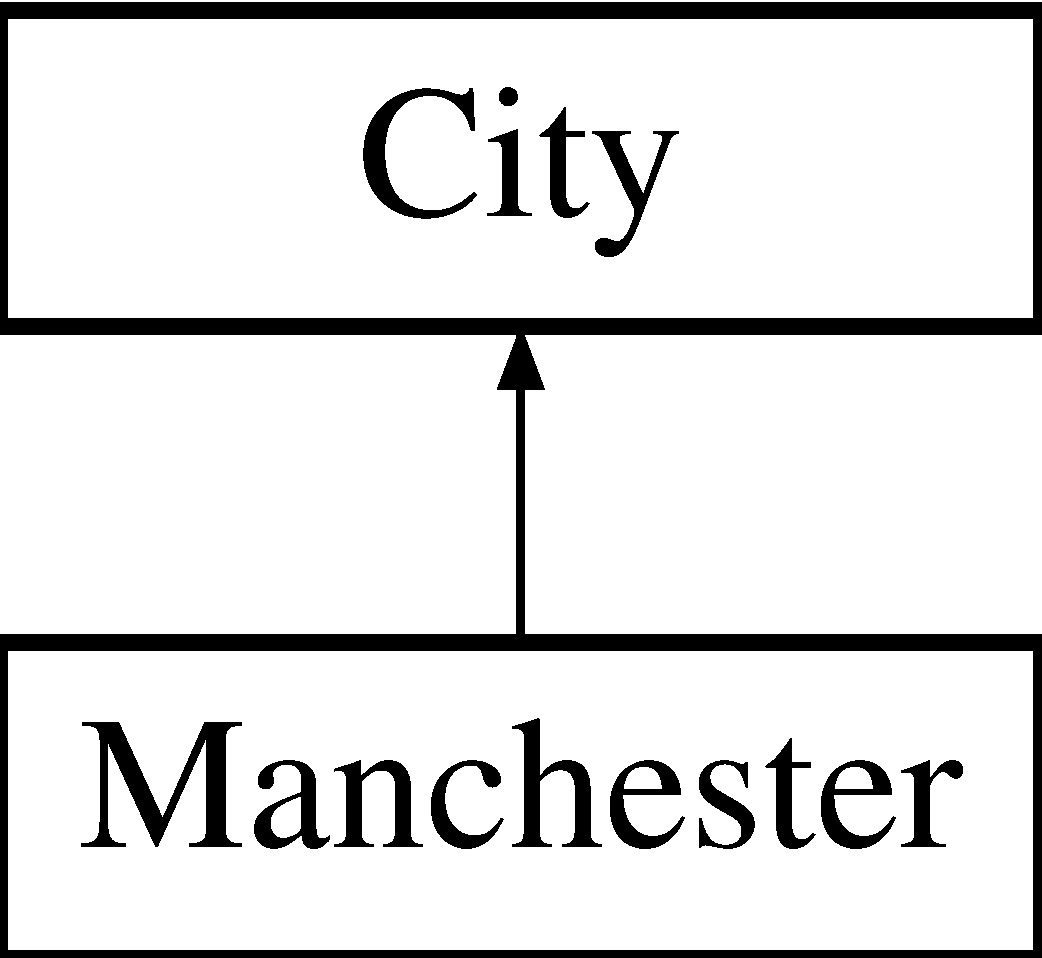
\includegraphics[height=2.000000cm]{class_city}
\end{center}
\end{figure}
\subsection*{Public Member Functions}
\begin{DoxyCompactItemize}
\item 
\hypertarget{class_city_a08e06bda79e81a069bad67791d993aa3}{}{\bfseries City} (std\+::string name, std\+::string info, double preference, double visit\+Time, double most\+Expensive\+Arrival\+Route)\label{class_city_a08e06bda79e81a069bad67791d993aa3}

\item 
\hypertarget{class_city_aad94270f6763e40fc8e27c5252e7bff3}{}double {\bfseries get\+Preference} ()\label{class_city_aad94270f6763e40fc8e27c5252e7bff3}

\item 
\hypertarget{class_city_a02cffba69dbd396bfa67e98ec5e3ff6f}{}double {\bfseries get\+Max\+Possible\+Travel\+Time\+Spent} ()\label{class_city_a02cffba69dbd396bfa67e98ec5e3ff6f}

\end{DoxyCompactItemize}
\subsection*{Public Attributes}
\begin{DoxyCompactItemize}
\item 
\hypertarget{class_city_afea8cd8800a8600fa54af37ac05bf177}{}std\+::string {\bfseries name}\label{class_city_afea8cd8800a8600fa54af37ac05bf177}

\item 
\hypertarget{class_city_a696817be4a02af25c9f05d16fc4f0646}{}std\+::string {\bfseries info}\label{class_city_a696817be4a02af25c9f05d16fc4f0646}

\item 
\hypertarget{class_city_a6077fb7eaa08209925af83a02c3a1c04}{}double {\bfseries preference}\label{class_city_a6077fb7eaa08209925af83a02c3a1c04}

\item 
\hypertarget{class_city_a9d651fe0145698c6210c40548e3e3977}{}double {\bfseries visit\+Time}\label{class_city_a9d651fe0145698c6210c40548e3e3977}

\item 
\hypertarget{class_city_a6373b5eb497338a81e5ffb377cacbf50}{}double {\bfseries most\+Expensive\+Arrival\+Route}\label{class_city_a6373b5eb497338a81e5ffb377cacbf50}

\end{DoxyCompactItemize}


The documentation for this class was generated from the following file\+:\begin{DoxyCompactItemize}
\item 
city.\+h\end{DoxyCompactItemize}

\hypertarget{struct_compare_nodes}{}\section{Compare\+Nodes Struct Reference}
\label{struct_compare_nodes}\index{Compare\+Nodes@{Compare\+Nodes}}


struct with comparison for nodes. Used in greedy\+Solve(). could help speedup search. not sure though...  




{\ttfamily \#include $<$brute\+Force.\+h$>$}

\subsection*{Public Member Functions}
\begin{DoxyCompactItemize}
\item 
\hypertarget{struct_compare_nodes_a2e5c79f8b055be389af6b4945e310474}{}bool {\bfseries operator()} (\hyperlink{class_brute_force__node}{Brute\+Force\+\_\+node} $\ast$a, \hyperlink{class_brute_force__node}{Brute\+Force\+\_\+node} $\ast$b)\label{struct_compare_nodes_a2e5c79f8b055be389af6b4945e310474}

\end{DoxyCompactItemize}


\subsection{Detailed Description}
struct with comparison for nodes. Used in greedy\+Solve(). could help speedup search. not sure though... 

The documentation for this struct was generated from the following file\+:\begin{DoxyCompactItemize}
\item 
brute\+Force.\+h\end{DoxyCompactItemize}

%--- End generated contents ---

% Index
\backmatter
\newpage
\phantomsection
\clearemptydoublepage
\addcontentsline{toc}{chapter}{Index}
\printindex

\end{document}
